\section{Introduction}


\label{introduction}
%Trace alignment is a well-known technique in conformance checking \cite{DBLP:conf/edoc/AdriansyahDA11} providing both a numerical assessment of the degree of conformance of a log trace with respect to a model, as well as a repair strategy if such trace does not conform to the given model. At the time of the writing,
%
In the existing literature on conformance checking, a common approach is based on trace alignment \cite{DBLP:conf/edoc/AdriansyahDA11}. This approach uses crisp process models as reference models. Yet, recently developed probabilistic conformance checking approaches provide a numerical quantification of the degree of conformance
%the existing approaches are used to check the degree of conformance
of an event log with a stochastic process model by either assessing the distribution discrepancies \cite{DBLP:conf/bpm/LeemansSA19}, or by exploiting entropy-based measures \cite{DBLP:conf/icpm/PolyvyanyyK19,DBLP:journals/tosem/PolyvyanyySWCM20}.
As these strategies are not based on trace alignments, these cannot be directly used to repair a given trace with one of the traces generated by a stochastic process model.
%As traces generated by such models are associated to a probability exhibiting its representativeness and relevance within the model, probabilistic trace alignment techniques should take into account the combined provision of trace probability and alignment cost.
%instead of finding trace alignments.
%
In this paper, we provide for the first time an approach for the probabilistic alignment of a trace and a stochastic reference
model. This approach is not comparable with the existing literature on probabilistic conformance checking as its output is not numeric but consists of a ranked list of alignments.
Providing different alignment options is useful since, conceptually, probabilistic trace alignment requires the analyst to
%handle the two possibly contrasting forces of the cost of the alignment on the one hand and the likelihood of the model trace with respect to which the alignment is computed.
%We consider the important tradeoff between both
%aspects.
balance between the likelihood of the model trace with respect to which the alignment is computed and the cost of the alignment.
%(if the cost of the alignment is too high even if the model trace is very likely applying too many changes in the original trace is in turn not very likely).

\begin{figure}[!t]
	\centering
	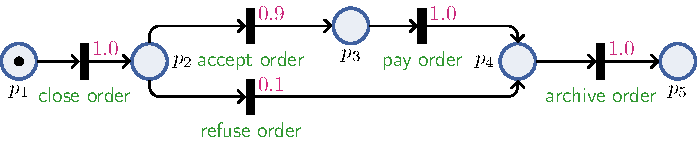
\includegraphics[width=.49\textwidth]{images/petri_tut.pdf}
	\caption{a simple Stochastic Workflow Net.}\label{fig:petri_tut}
	%\vspace{-1.4cm}
\end{figure}
%For example, the probabilistic alignment of a trace with a stochastic net could be represented by the model trace maximizing the combined provision of minimum trace alignment cost and maximum model trace probability.
With reference to Figure~\ref{fig:petri_tut}, a user might be interested to align the log trace $\langle \textsf{close order},\,\textsf{archive order}\rangle$ with one of the two possible model traces $\langle\textsf{close order},$ $\textsf{accept order},\,\textsf{pay order},\,\textsf{archive order}\rangle$ or $\langle$\textsf{close order}, \textsf{refuse order}, \textsf{archive order}$\rangle$. While the latter trace provides the least alignment cost though the model trace has a low probability ($0.1$), the former gives a slightly greater alignment cost while providing a higher model trace probability ($0.9$). Since, depending on the context, analysts might prefer either the former or the latter alignment, providing a selection of the best $k$ alignments among all the distinct model traces empowers the analysts to find their own trade-off between alignment cost and model trace probability.
%However, in some cases, the user could prefer to identify an alignment with a lower cost even if based on a less probable model trace, while, in other cases, the user could favor a model trace with a higher probability at the expense of a higher alignment cost. Therefore, to provide users with an instrument that allows them to find their own trade-off between alignment cost and model trace probability, we need to return the best $k$ alignments among all the distinct model traces.


%Since when aligning an event log with a stochastic net distinct model traces have different probabilities, the retrieval of the best model trace maximizing the combined provision of minimum trace alignment cost and maximum model trace probability might not suffice. In some cases, indeed, the user could prefer to identify an alignment with a lower cost even if based on a less probable model trace, while, in other cases, the user could favor a model trace with a higher probability at the expense of a higher alignment cost. We consider, therefore, the important tradeoff between both aspects.
%Therefore, in this paper, we propose trace alignment approaches that return the best

To do this, we frame the probabilistic trace alignment problem into the well-known $k$-Nearest Neighbors ($k$NN) problem \cite{Altman} that refers to finding the $k$ nearest data points to a \textit{query}  from a set  of \textit{data points} via a distance function.
We introduce two ranking strategies. The first one is based on a brute force approach that reuses existing trace aligners such as \cite{DBLP:conf/edoc/AdriansyahDA11,LeoniM17}, where the (optimal) ranking of the top-k alignments is obtained by computing the Levensthein distance between the trace to be aligned and all the model traces and by multiplying each of these distances by the probability of the corresponding model trace. However, even if this approach returns the best trace alignment ranking for a query trace, the alignments must be computed a-new for all the possible traces to be aligned. For models generating a large number of model traces, this would clearly become unfeasible. Therefore, we propose a second strategy that produces an approximate ranking where traces are represented as numerical vectors via an embedding. {Then, by exploiting ad-hoc data structures,
	%such as Vp-Trees \cite{Fu2000}, Kd-Trees \cite{Maneewongvatana99}, and M-Trees \cite{Ciaccia},
	we can retrieve the neighborhood of size $k$ containing the traces similar to the given query  by pre-ordering (\textit{indexing}) the model traces  via the aforementioned distance.
	%Thus, we do not need to analyze the entire space, but just start the search from the top-$1$ alignment.
	If the embeddings for our model traces are independent of the query of choice, this would not require to constantly recompute the numeric vector representation for the model traces.
	%	
	
	%%%%% Proposed part as the last part of the introduction:
	%\texttt{\color{red}[TODO]}
	%\todo{this is too specific for an introduction; in particular, too many details on how the experiments are done.}
	We implemented both strategies and perform experiments using a real life event log coming from a hospital system to empirically evaluate their properties. We assess the two strategies as follows:
\begin{mylist}
	\item first, we evaluate the degree of approximation introduced by the approximate-ranking approach if compared with the optimal-ranking (\S\ref{subsec:apprp}).
	\item Then, we evaluate the computational time required to produce the top-k alignments with the two strategies (\S\ref{subsec:efficio}). We observe that approximate-ranking alignments provide the best trade-off between accuracy and efficiency.
\end{mylist}

\begin{figure*}[!t]
	\begin{minipage}{.49\textwidth}
		\centering
		\includegraphics[width=.7\textwidth]{images/petri.pdf}
		\caption{A sample \uswn $N$. Labels are shown in green, $\tau$ transitions in grey, weights in magenta.}\label{fig:spn}
	\end{minipage}\hfill \begin{minipage}{.49\textwidth}
	\centering
		\includegraphics[width=.7\textwidth]{images/rg.pdf}
		\caption{Reachability graph  of the \uswn $N$. Probabilities are shown in violet.}\label{fig:rg}
	\end{minipage}

	\begin{minipage}{.4\textwidth}
		\centering \includegraphics[width=.7\textwidth]{images/running_example.pdf}
		\caption{Preliminary Transition graph $TG$ encoding the SWN $N$ with no $\tau$-closures.}\label{fig:lmc}\label{fig:orig}
	\end{minipage}\hfill \begin{minipage}{.4\textwidth}
	\centering \includegraphics[width=.7\textwidth]{images/closed_example.pdf}
		\caption{Transition graph $TG$ resulting from $N$ after $\tau$-closure.}\label{fig:closed}
	\end{minipage}
	\vspace{-.6cm}
\end{figure*} 